\chapter{Le modèle en couches}
\section{Introduction}
Le but de ce modèle est de décrire les propriétés des états fondamentaux (spin, parité, moments dipolaire, 
quadrupolaires, \dots). Il a aussi pour but d'expliquer l'orgine des nombres magiques ($2,8/,20,2/8,50,82,126)$. 
Ceux-ci ont des propriétés intéressantes
\begin{itemize}
\item[$\bullet$] Nombre de neutrons/protons donnant des propriétés particulières au noyau
\item[$\bullet$] Grande énergie de liaison et énergie d'excitation élevée
\item[$\bullet$] Effets microscopiques (absents des modèles collectifs) et petit rayon
\end{itemize}

L'Hamiltonien exact s'écrit
\begin{equation}
H = \sum_{i=1}^A T_i +\sum_{i=1}^A\underbrace{\sum_{j=1}^A v(r_i-r_j)}_{\approx U_i(r_i)}
\end{equation}
Celui-ci est alors remplacé par
\begin{equation}
H = \sum_{i=1}^A (T_i+U_i(r_i)) + H_{res}
\end{equation}
où $H_{res}$ est un Hamiltonien "résiduel" supposé négligeable. Cet Hamiltonien est à particules indépendantes et
chaque nucléon ressent un potentiel moyen généré par les autres nucléons. En négligeant le terme résiduel, nous
avons la forme d'un Hamiltonien séparable : le problème à $A$ nucléons a été changé en $A$ problèmes à $1$ 
nucléon
\begin{equation}
H = \sum_{i=1}^A H_i,\qquad\qquad E = \sum_{i=1}^A E_i, \qquad\qquad \Psi = \Phi_1\dots\Phi_A
\end{equation}

Différentes approximations sont possibles pour le potentiel $U(r_i)$. Par exemple, l'interaction de \textsc{Coulomb}
étant faible par apport à l'interaction nucléaire, nous allons négliger \textsc{Coulomb}. Généralement, $U_i$ tend
alors vers zéro et tend à être attractif à courte portée (forme typique d'un potentiel nucléaire). Mais un tel
potentiel n'ayant pas de solution analytique, il va falloir ruser.


\subsection{A. L'oscillateur harmonique}
Dans le cas d'un oscillateur à une dimension $x$, nous avons $U(x) = \frac{1}{2}m\omega^2x^2$. On peut écrire
\begin{equation}
\left(\frac{\hbar^2}{2m}\frac{d^2}{dx^2} + \frac{1}{2}m\omega^2x^2\right)\phi(x) = E\phi(x)\quad\Leftrightarrow
\quad \left(-\frac{d^2}{dx^2}-\frac{m\omega^2}{\hbar^2}x^2\right)\phi(x) = \frac{2mE}{\hbar^2}\phi(x)
\end{equation}
On peut trouver $b^4 = \hbar^2/(m^2\omega^2)$ (où $b$ est le paramètre d'oscillateur). En posant
\begin{equation}
\phi(x) = \exp(-x^2/2b^2)\tilde{\phi}(x)
\end{equation}
On peut trouver les énergies et les fonctions propres
\begin{equation}
E_n(x) = \hbar\omega\left(n+\frac{1}{2}\right),\qquad\qquad \phi_n(x) \propto \exp(-x^2/2b^2) H_n(x/b)
\end{equation}
où $H_n(x)$ sont les polynômes d'\textsc{Hermitte}.

\begin{center}
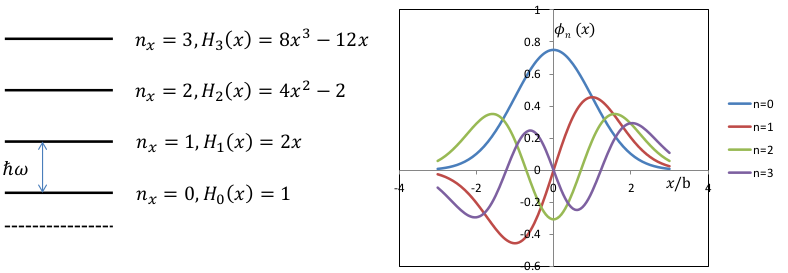
\includegraphics[scale=0.5]{ch9/image1}
\captionof{figure}{ }
\end{center}

La chose fantastique est que le passage en trois 
dimension se fait en sommant les hamiltonien pour chaque dimension. L'énergie est alors donnée par
\begin{equation}
E_{n_x,n_y,n_z} = \hbar\omega\left(n_x+n_y+n_z+\frac{3}{2}\right)
\end{equation}
Pour $n_x=n_y=n_z=0$ il n'existe qu'un seul état possible. Par contre, si l'un deux vaut 1 nous avons
trois états possible. Ceci est la dégénérescence des états, la même énergie est commune à un certain nombre
d'états différents.\\



La dégénérescence (valant toujours 1 dans le cas 1D) est donnée par
\begin{equation}
N_n = \sum_{n_x=0} (n-n_x+1) = \frac{(n+1)(n+2)}{2}
\end{equation}

Les \textit{slides 18} et \textit{19} reprennent ces résultats dans le cas des coordonnées sphériques. On retrouve
au final trois fonctions d'ondes aux coordonnées sphériques qui correspondent aux trois trouvées dans les
coordonnées cartésiennes.\\

	\begin{wrapfigure}[9]{l}{8.5cm}
	\vspace{-5mm}
	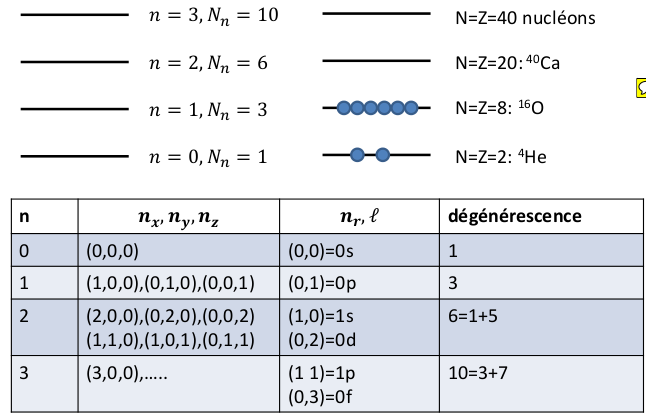
\includegraphics[scale=0.35]{ch9/image2}
	\captionof{table}{ }
	\end{wrapfigure}

Cette dégénérescence compte le nombre de nucléon que l'on peut mettre par niveau. Sur le niveau 0 on peut en
mettre 2, sur le niveau 1 on peut en mettre 6, \dots Il y a chaque fois un facteur deux venant du spin. Si
l'énergie de liaison est grande, c'est parce qu'une couche est fermée : on retrouve bien 2 le premier nombre 
magique (qui correspond à une couche pleine). \\

En effet, si une couche est remplie, rien ne se passera si l'énergie de liaison n'est pas fournie : nombre 
magique. Par contre, si la couche n'est pas remplie il peut y avoir réorganisation au sein de celle-ci. Ce 
modèle permet d'expliquer les trois premiers nombres magiques (2,8,20) grâce à cette explication mais plus les
suivants (40 est prédit comme nombre magique dans cette théorie mais ça ne colle pas expérimentalement). Il 
manque donc quelque chose à ce modèle!

\subsection{B. Puits infini}
Un autre potentiel que l'on peut considérer est celui du puits infini
\begin{equation}
\left\{\begin{array}{lll}
U(r) &= 0&\qquad\text{ pour } r< a\\
U(r) &= \infty&\qquad\text{ pour } r\geq a
\end{array}\right.
\end{equation}
Ce potentiel suit tout de même une certaine logique. Au delà du noyau il n'y a pas de potentiel, tous les 
nucléons restent à l'intérieur du noyau. En considérant un tel potentiel, on trouve des énergies s'exprimant
via les séries de \textsc{Bessel}. 
\begin{equation}
E_{n_r,\ell} = \frac{\hbar^2}{2ma^2}x^2_{n_r,\ell}
\end{equation}
où $x_{n_r,\ell}$ est le numéro $n_r$ de la fonction de \textsc{Bessel} sphérique $j_\ell(x_{n_r,\ell})$. \\

	\begin{wrapfigure}[10]{l}{8.5cm}
	\vspace{-5mm}
	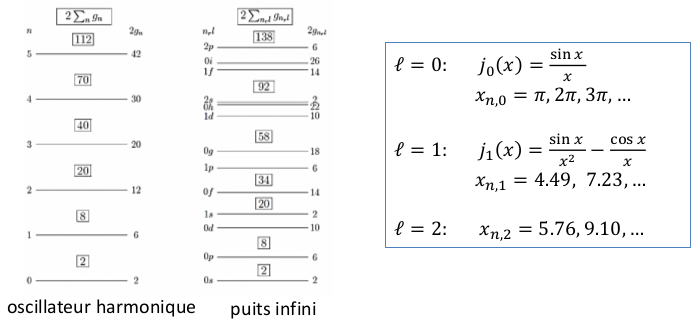
\includegraphics[scale=0.34]{ch9/image3}
	\captionof{figure}{ }
	\end{wrapfigure}
Comme l'équation est du second ordre, il existe forcément deux solutions linéairement indépendantes donnant lieu à
une dégénérescence $2(2\ell +1)$ (voir ci-contre). En exprimant les énergies à partir de $k_a$, $j_l(k_a)=0$ 
signifie que $k_a$ doit être égal au zéro de ces fonctions de \textsc{Bessel}. Malheureusement, ce potentiel
ne prédit correctement que les trois premiers nombres magiques.


\subsection{C. Potentiel de Woods-Sakon}
Il s'agit d'un potentiel plus réaliste pour lequel il n'existe pas de solution analytique (calcul numérique). 
Malgré l'introduction d'une diffusivité, ce potentiel ne fait pas mieux que les deux précédents. Il y a 
forcément une contribution qui a été oubliée : il s'agit d'un terme de spin-orbite.


\subsection{D. Potentiel de spin-orbite}
Afin de tenter de régler le problème, nous allons introduire un potentiel de spin-orbite
\begin{equation}
U(r) = U_0(r)+V_{SO}(r)\vec\ell.\vec s
\end{equation}
L'introduction du spin fait que $\ell$ et $s$ ne sont plus de bon nombres quantiques
\begin{equation}
[U,\ell^2] \neq 0,\qquad\qquad\qquad [U,s^2]\neq 0
\end{equation}
Cependant, le nombre quantique de moment cinétique total $j$ est lui un bon nombre quantique
\begin{equation}
[U,j^2]=0
\end{equation}
Il est dès lors nécessaire d'obtenir des fonctions d'ondes à partir du couplage entre $l$ et $s$. Nous allons
avoir des fonctions d'ondes
\begin{equation}
\ket{n_n l j m} = \sum_{m_lm_s} \bra{l m_l \frac{1}{2} m_s}\ket{jm}\ket{1/2 m_s}
\end{equation}
Nous allons associer une énergie à chacune de ces fonctions d'ondes. En adoptant une notation efficace, 
on peut trouver l'énergie de la partie spin-orbite
\begin{equation}
\bra{jm} \vec l . \vec s\ket{jm}
\end{equation}
Sachant que $j^2 = (\vec l + \vec s)^2$, on trouve
\begin{equation}
1/2\bra{jm} \vec j^2-\vec l^2-\vec s^2 \ket{jm}
\end{equation}
où $j = l\pm 1/2$.\\

	\begin{wrapfigure}[14]{r}{5.5cm}
	\vspace{-5mm}
	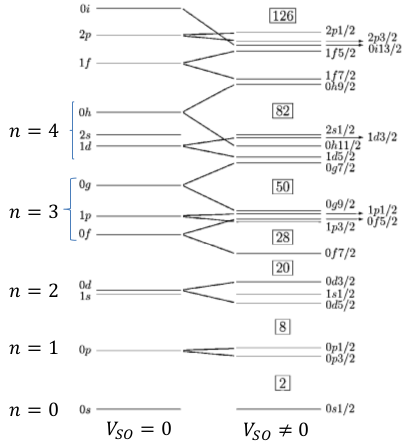
\includegraphics[scale=0.37]{ch9/image4}
	\captionof{figure}{ }
	\end{wrapfigure}
	
 En explicitant les valeurs propres
\begin{equation}
1/2\bra{jm}  j(j+1)-s(s+1)-3/4  \ket{jm}
\end{equation}
Si $j = l+1/2 \rightarrow 1/2[-l+1/2)(l+3/2)-l(l+1)-3/3] = l/2$ et si $j=l-1/2 \rightarrow -1/2(l+1)$. Le 
terme spin-orbite cause donc une levée de la dégénérescence en $\ell$ des niveaux. En effectuant la différence
entre les deux
\begin{equation}
E(l+1/2)-E(l-1/2) = 1/2(2l+1)
\end{equation}
On constante que la levée de la dégénérescence va être d'autant plus forte que $\ell$ est grand. Le résultat est
sans appel car les nombres magiques 2,8,20,28,50,82 et 126 sont en accord avec l'expérience (pour une couche
fermée ($J=0$)).\\

\danger\ Nous avons adopté la notation $n_r \ell_j$ (exemples : $0s_{1/2}, 0p_{1/2},\dots$) pour différencier
les couches.


\section{Spin et parité de l'état fondamental du noyau}
Dans le noyau, le spin $J$ est défini par le couplage de tous les spins individuels $j$ tandis que la parité
$\pi$ est définie par les produits des parités individuelles $(-1)^\ell$. Nous allons ici utiliser le 
\textbf{modèle en couches extrême} qui considère que les nucléons forment des paires de spin 0.

\subsubsection*{Noyaux pairs-pairs ($N, Z$ pairs) : spin entier}
Dans un tel noyau, le \textbf{spin et la parité} sont $J=0^+$. Le modèle en couches extrême est quasiment
toujours vérifié et il permet de justifier la grande énergie d'excitation des noyaux magiques. 

\subsubsection*{Noyaux pairs-impairs ($N$ ou $Z$ impair) : spin demi-entier}
Cette fois-ci le spin est donné par le spin du dernier nucléon (c'est souvent le nucléon célibataire qui donne
ses propriétés au noyau) : $J=j$. La parité est donnée par $\pi = (-1)^\ell$.\\

Le noyau $^{17}$O est formé du cœur $^{16}$O et d'un nucléon qui est sur $0d_{5/2}$. A partir du modèle en couche,
on peut prédire en connaissant le schéma des niveau) le spin de l'état fondamental qui est de $J=5/2^+$.\\


	\begin{wrapfigure}[10]{r}{3.5cm}
	\vspace{-8mm}
	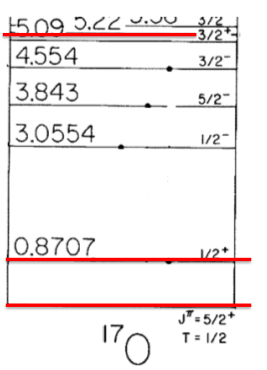
\includegraphics[scale=0.37]{ch9/image5}
	\captionof{figure}{ }
	\end{wrapfigure}
	
En effet, considérons le modèle extrême avec $Z=8, N=9$. Regardons la divisions des niveaux\footnote{Revoir}
\begin{description}
\item[N=0] Une seule division
	\begin{itemize}
	\item $0s_{1/2}$ : on y place deux nucléons
	\end{itemize}
	
\item[N=1] Deux divisions
	\begin{itemize}
	\item $0p_{3/2}$ : on y place quatre nucléons
	\item $0p_{1/2}$ : on y place deux nucléons	
	\end{itemize}	
	
\item[N=1] Trpos divisions
	\begin{itemize}
	\item $0d_{5/2}$ : on y place un nucléon
	\item \dots 
	\end{itemize}		
\end{description}


Le modèle en couche permet ainsi d'expliquer l'état excité (nucléon $0s_{1/2} \to J=1/2^+$) mais aussi les
états $5/2^+,1/2^+,3/2^+$ (en rouge dans le spectre). Pour les autres états, c'est plus compliqué.


\subsubsection*{Autres exemples}
Le \textit{slide 27} donne d'autres exemples. Le $^{39}$K ($Z=19,N=20$) possède une couche $sd$ complète mais
présente un "trou" dans la douche $sd_{5/2}$. En enlevant une particule dans le couche $d_{3/2}$, le dernier 
nucléon célibataire aura un moment cinétique $J=3/2^+$, soit le spin de l'état fondamental\footnote{Il faudrait
plus de notes, je vois pas trop pourquoi ces états la sont justifiés et pas les autres ni même la conclusion
retirée ici.}


\subsubsection*{Noyaux plus lourds}
Le modèle en couche permet également d'expliquer les noyaux lourds (voir \textit{slide 28} et \textit{29}).


\section{Modèle en couches à plusieurs particules}
Considérons un "cœur" ainsi que quelques neutrons supplémentaires. Il y a nécessite d'obtenir plusieurs fonctions
de bases (via une diagonalisation de l'hamiltonien). En effet, $J=1$ donne une fonction, $J=1$ en donne cinq 
(soit le nombre de projection) et $J=2$ en donne 9. La somme $1+5+9=15$ est le nombre de fonction d'onde avec 
lesquelles nous avons travaillés. \\

Regardons le spectre de $^{18}$O pour les neutrons et les protons. Il s'agit d'un cœur de $^{16}$O avec deux
neutrons dans le couche $0d_{5/2}$. On remarque l'existence de trois états ($0^+, 4^+, 2^+$) d'énergie 
relativement proche. En pratique on ne retrouve pas la dégénérescence attendue : cela vient du fait que
$H_{res}$ a été négligé


	\begin{center}
	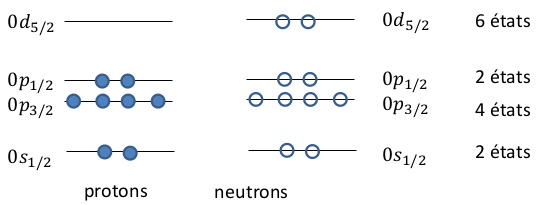
\includegraphics[scale=0.37]{ch9/image6}
	\captionof{figure}{Deux neutrons pour six états possibles donne bien $(6*5)/2=15$ états possibles. Les 
	fonctions d'ondes totales sont obtenues par couplage de deux moments cinétique $5/2$. Elles sont bien
	antysymétrique ($J=0,2,4$ (on retrouve bien les 15 fonctions $1+5+9=15$)).}
	\end{center}

Considérons le $^{18}$F. La symétrie que nous avions précédemment imposée n'a plus de raison d'être : il y a
six fonctions pour les neutrons et de même pour les protons donnant un total de 36 fonctions ($1+3+5+7+9+11=
36$, le compte est bon!). On aura dans le bas du spectre de $^{18}$F six état allant de $0^+$ à $5^+$. Chacune
de ces fonctions sont des déterminants de \textsc{Slater} basés sur l'hamiltonien de l’oscillateur harmonique
comme décrit au \textit{slide 31}.



\section{Extension aux couches supérieures}
En considérant les couches $0d_{5/2}, 1s_{1/2}$ et $0d_{3/2}$, il est possible de décrire 12 états et d'avoir
alors $C^{12}_2=66$ fonctions. Ceci permet d'améliorer la description de l'état fondamental tout simplement
en décrivant plus d'état. \\

Plus on augmente l'espace, plus on a de fonctions. Le nombre de fonction monte assez vite (avec $N, Z$) et on 
peut arriver au \textit{No core shell model} où on suppose qu'il n'y a pas de cœur rempli si le nombre 
de fonctions est de l'ordre du milliard !

\vspace{4cm}
\begin{center}

\includegraphics[scale=0.2]{ch9/fin}
\end{center}